\documentclass[12pt,a4paper]{article}
\usepackage[utf8]{inputenc}
\usepackage[T1]{fontenc}
\usepackage{amsmath}
\usepackage{amsfonts}
\usepackage{amssymb}
\usepackage[english]{babel}
\usepackage{array}
\usepackage{tabularx}
\usepackage{tikz}
\usepackage{ebproof}
\usepackage{listings}
\usepackage{graphicx}
\usepackage{url}
\author{ANDREI-ALIN CORODESCU}
\title{Program Equivalence : A Relational Separation Logic interactive prover implemented in Maude}
\newcommand{\hq}[4]{
	\left\{{#1}\right\}
	\let\scriptstyle\textstyle 
	\substack{{#2} \\ 	\let\scriptstyle\textstyle {#3}} 
	\left\{{#4}\right\}
}

\newcommand{\stoptocwriting}{%
	\addtocontents{toc}{\protect\setcounter{tocdepth}{-5}}}
\newcommand{\resumetocwriting}{%
	\addtocontents{toc}{\protect\setcounter{tocdepth}{\arabic{tocdepth}}}}
\usepackage{color}

\definecolor{codegreen}{rgb}{0,0.6,0}
\definecolor{codegray}{rgb}{0.5,0.5,0.5}
\definecolor{codepurple}{rgb}{0.58,0,0.82}
\definecolor{backcolour}{rgb}{0.95,0.95,0.92}
\lstdefinestyle{mystyle}{
	backgroundcolor=\color{backcolour},   
	commentstyle=\color{codegreen},
	keywordstyle=\color{magenta},
	numberstyle=\tiny\color{codegray},
	stringstyle=\color{codepurple},
	basicstyle=\footnotesize,
	breakatwhitespace=false,         
	breaklines=true,                 
	captionpos=b,                    
	keepspaces=true,                 
	numbers=left,                    
	numbersep=5pt,                  
	showspaces=false,                
	showstringspaces=false,
	showtabs=false,                  
	tabsize=2
}

\lstset{style=mystyle}
\begin{document}
\begin{titlepage}
\begin{center}
\textbf{
ALEXANDRU IOAN CUZA UNIVERSITY OF IAȘI
}
\\
\textbf{FACULTY OF COMPUTER SCIENCE}
\end{center}
   \vspace{40mm}
\begin{center}
	\Large\textbf {Program Equivalence: An Interactive Relational Separation Logic Prover Implemented in Maude}\\
	\vspace{40mm}
	\large\textit {ANDREI-ALIN CORODESCU}
	\\
	\vspace{20mm}
	\textbf{Session: }\textit{July, 2018}\\
	\vspace{30mm}
	\textbf{Scientific Coordinator}\\
	\textbf{\textit{Conf. Dr. Ciobâcă Ștefan}}
	\vspace{30mm}
\end{center}
\end{titlepage}
\begin{abstract}
	Lucrarea de fata descrie procesul de dezvoltare a unui utilitar interactiv utilizat in analiza formala a programelor, folosindu-se de Logica Separatoare Relationala \cite{relational} si Logica Separatoare \cite{primer} \cite{SeparationLogic}, utilizand Maude \cite{maudesite} drept cadru de dezvoltare. Componenta interactiva se imbina cu o componenta automatizata, prin care parti din demonstratie vor fi realizate automat. Lucrarea este orientata pe rezolvarea problemei prin intermediul functionalitatilor oferite de Maude si va include secvente de cod ce vor ilustra conceptele cheie in modelarea si aplicarea fundamentelor teoretice.
\end{abstract}
\pagebreak
\tableofcontents
\pagebreak
\section*{Introduction}
The present paper describes the development of an interactive tool for reasoning how to programs are related, based on studied and previously used theoretical concepts and technologies which facilitate the implementation. \\

The tool represents an implementation of Hoare Logic - which allows formal reasoning about a program - , along  with 2 of its extensions, namely the Separation Logic (named Separation Logic from now on) and Relational Separation Logic \cite{relational} (named Relational Logic from now on). The 2 extensions simplify the Hoare Logic proofs, mainly using the "*" connector, allowing for local reasoning of effects of statements in a program . The tool has been implemented in Maude, a high performance logical framework with powerful metalanguage applications which facilitate the implementations of executable environments for logics.\\

The tool is built as a CLI which helps \cite{primer} \cite{SeparationLogic} \cite{JAVAITP} \cite{REWRITING} \cite{maudeprimer} \cite{manual} \cite{rewrConcurrency} \cite{cyclist} with reasoning how two programs are related using Relational Separation Logic specifications. As a consequence of the dependency of Relational Separation Logic on Separation Logic, proofs about single programs using the latter are also supported by the tool. The tool has been developed with extensibility in mind, the main desired extensions being concurrent programs support and automatic proofs. \\

The rest of the paper is organized as follows: 
\begin{itemize}
	\item {\textbf{Section 1} will describe the main personal contributions to the realization of this project}
	\item {\textbf{Section 2} will present the problem this project aims to solve}
	\item {\textbf{Section 3} will shortly present some other projects related to ours}
	\item {\textbf{Section 4} will briefly touch upon the theoretical foundations of this project, together with the technologies used to implement them}
	\item {\textbf{Section 5}, the main section of this paper, will present our approach to solving the problem, and discuss how it can be improved in the future. All the elements of our project will be presented in an individual sub-section}
\end{itemize}
\section{Contributions}
Personal contributions to the realization of the project : 
\begin{itemize}
	\item Modelled the Relational Logic and Separation Logic using Maude equational and rewriting logic specifications . 
	\item Developed an interactive tool for reasoning about program behaviour using the aforementioned logics.
	\item Automation of some tasks which makes the tool more convenient to use .
	\item Examples of formal proofs done using the tool
\end{itemize}
\section{Description of the problem}
The problem this project is aiming to solve is related to formal reasoning about the execution of code, mainly focusing on how two programs are related to each other (most often the relation to be proven is equivalence)\\

Comparing programs or code fragments and studying their equivalence is part of every software engineer's activities when they are testing an alternative implementation for an existing solution, fixing bugs, launching new product versions, etc . Naturally, for every process completed manually there are efforts being made in order to make it more efficient, less error-prone and, in the end, automate the process all together. Once such a task is automated in software engineering, it can be included in the flow of any research or development phase of a product. An example benefiting from a formal proof of program equivalence is compiler optimization, where the optimized code needs to be equivalent to the input one . \\

This project aims to lay the foundations of a tool which facilitates formal reasoning on the way two programs are related with a focus on extensibility and automation of tasks.

\section{Previous work}
Previous work related to the topic has been done mostly in terms of Separation Logic based tools, with Relational Separation Logic not being treated as much. \\

A notable example which also uses the same framework as this project, namely Maude, is the Java+ITP\cite{JAVAITP} tool, which enables analysis of Java programs using Separation Logic. The implementation relies heavily on Maude's ITP (iterative theorem prover).

\section{Theoretical Foundations and technologies}
This section will briefly introduce the concepts on which the project is based, together with the technologies used to implement it, along with a few references to resources which explain them in depth.
\subsection{Separation Logic}
Separation Logic allows for reasoning about the effects of code on the program state in a formal manner. The main abstraction used in separation logic is the \textbf{Hoare Triple}
\[ \{P\}\  C\  \{Q\} \]
where \(P\) denotes the a condition satisfied by state of the program before the execution of the command \(C\) and \(Q\) denotes another condition satisfied by state of the program after the execution of \(C\).
\\

Good references for reading on separation logic include : 
\begin{itemize}
	\item \cite{primer} - for a good introduction and some interesting usages
	\item \cite{SeparationLogic} - for a more in depth explanation, including the mathematical fundaments of the logic
\end{itemize} 
\subsection{Relational Separation Logic}
Relational Separation Logic, which is the central concept of our project builds upon the Separation Logic to reason about how to programs are related, by using the concept of a \textbf{Hoare Quadruple}
\[\{R\}\ {C_1 \atop C_2}\   \{T\}\]
\(R\) represents a \textbf{relation} between the two program states holding before the execution of commands \(C_1\) and \(C_2\) respectively while \(T\) represents a \textbf{relation} which holds after the execution of the two commands. 
\\

Relational Separation Logic is presented in detail in \cite{relational}.
\subsection{Maude}
Maude \cite{maudesite} is a framework based on rewriting logic \cite{rewritingLogic} which allows for natural representations of a wide range of applications, including other logics, which made it a perfect fit for our case. Maude allows for short and simple, yet clever and self-explanatory solutions to problems. 
\\

 Good references for Maude language include:
 \begin{itemize}
 	\item Maude Primer \cite{primer} which was written for Maude 2.0.1 but still applies to the latest versions of Maude is a good starting point for learning Maude, as it introduces the language in a more informal, friendlier way
 	\item Maude Manual \cite{manual} which presents the whole Maude system in depth, along with the mathematical foundations
 	\item All about Maude book \cite{allAboutMaude} which includes everything contained in the manual and presents some of the more relevant tools implemented in Maude .
 \end{itemize}
\section{Relational Separation Logic Interactive Prover} 
This section will include details related to the implementation and usage of the Relational Separation Logic prover and highlight a few of Maude's features which made it the a language fit for the purpose of this project.
\\

The information presented in this section assumes the reader's familiarity with Maude, especially the META-LEVEL module and with the underlying theoretical concepts implemented by the prover (Separation Logic and Relational Separation Logic). References for these can be found in the previous section.
\\

This section will include snippets of Maude code, but since Maude is a very expressive and self-explanatory language, I have not included of thorough presentation of every language construct defined for the scope of this project. Ideas presented will be accompanied by some examples and key ideas of the implementation but for a more detailed presentation, please refer to the code itself.
 
\subsection{Modelling the Separation Logics}
Thanks to Maude's ability to naturally represent logics, the modelling of the Separation Logic and Relational Separation Logic is mostly reduced to translating the logical formulae into appropriate syntax for Maude, making the representational distance (the amount of information lost when representing a theoretical concept into a programming language)\cite{manual} almost non existent. \\

Each proof rule in the Separation Logic and Relational Separation Logic has been translated into a Maude rewrite rule. 
\\
The prover is centered around the concept of \textbf{Goals} which can be one of the three things: 
\begin{itemize}
	\item {Hoare Quadruple} - corresponding to Relational Separation Logic
	\item {Hoare Triple} - corresponding to Separation Logic
	\item {Implication between relations / assertions} 
\end{itemize} 
The proof rules are interpreted in a bottom-up manner, meaning that applying a rule to a goal matching the conclusion of a rule will generate new goals consisting of the hypothesis elements of the rule : Figure \ref{fig:SLTranslation} presents how a Separation Logic rule has been translated into Maude syntax and Figure \ref{fig:RSLTranslation} presents the same process for the Relational Separation Logic counterpart of the rule.
\begin{figure}[h]
	Consequence Rule
	\medskip
	\[
	\begin{prooftree}
	\Hypo{P \Rightarrow P\prime}
	\Hypo{\{P\prime\} C \{Q\prime\}}
	\Hypo{Q \Rightarrow Q\prime}
	\Infer 3 {\{P\}\  C  \{Q\}}
	\end{prooftree}	
	\]
	Is represented in Maude syntax as : 
\begin{lstlisting}[caption=Separation Logic Consequence rule]
	rl [SeparationLogic-Consequence] : {P} C {Q} => ((P => P1) <> ({P1} C {Q1})) <> (Q1 => Q) [nonexec] .
\end{lstlisting}
	\caption{Example of a translation to Maude syntax of a Separation Logic proof rule}
	\label{fig:SLTranslation}
\end{figure}

\begin{figure}[h]
	Consequence Rule
	\[
	\begin{prooftree}
	\Hypo{R \Rightarrow R_1}
	\Hypo{\hq{R_1}{C}{C\prime}{S_1}}
	\Hypo{S \Rightarrow S_1}
	\Infer 3 {\hq{R}{C}{C\prime}{S}}
	\end{prooftree}	
	\]
	Is represented in Maude syntax as : 
	\begin{lstlisting}[caption=Relational Separation Logic Consequence rule]
	rl [Consequence] : { R } C1 -- C2  { S } => ((R => R1) <> ({R1} C1 -- C2 {S1})) <> (S1 => S) [nonexec] .
	\end{lstlisting}
	\caption{Example of a translation to Maude syntax of a Relational Separation Logic proof rule}
	\label{fig:RSLTranslation}
\end{figure}
The \texttt{<>} operator is used to separate sub-goals generated by the rule.
\\

The \texttt{---} operator is used to separate the two snippets of code mentioned in the \textbf{Hoare Quadruple}.
\\

All the rules are marked with the attribute \texttt{[nonexec]} because we want them to be applied in a controlled manner, at the meta-level. Some of the rules, the examples included, are not even valid executable Maude rules, because they make use of variables before binding them (for example \texttt{P1} is used in a rule before it is bound). At the meta-level however we can manually bind values to those variables, as we will exemplify when discussing how we apply these rules to goals.
\subsubsection{Sort Hierarchy}
Much in the same manner as we modeled the language grammar, the Relational Separation Logic \cite{relational} and Separation Logic \cite{SeparationLogic} \cite{primer} have been modeled by defining sorts and declaring operators using these sorts. The main point of reference for our modeling has been \cite{relational}, for both logics. Some examples of translations from specification to code are included below.
\begin{itemize}
	\item \texttt{Assertion} is the sort used to handle Separation Logic assertions. It is a super sort of the \texttt{BExp} sort defined as part of our language.
	\item \texttt{HoareTriple} is the sort associated with the concept with the same name, in a Separation Logic context.
	\begin{lstlisting}[caption=Hoare Triple constructor operator]
op {_}_{_} : Assertion Command Assertion -> HoareTriple .\end{lstlisting}
	\item \texttt{Relation} is the sort associated with Relational Separation Logic relations. As it was the case with \texttt{Assertion}, it is a super sort of the \texttt{BExp} sort of our language grammar. Because both the \texttt{Relation} and \texttt{Assertion} are super sorts of the same sort, Maude will display a few warnings which are not affecting functionality, but in the future, creating a separate \texttt{BExp} sort for both the \texttt{Assertion} and \texttt{Relation} sorts would be a better option.
	\item \texttt{HoareQuadruple} is again associated with the concept with the same name, in the Relational Separation Logic context.
	\begin{lstlisting}[caption=Examples of Relational Separation Logic specific constructs]
--- Operator which creates a relation from two assertions
op [_;_] : Assertion Assertion -> Relation .
--- Operator which constructs a Hoare Quadruple 
op {_}_--_{_} : Relation Command Command Relation -> HoareQuadruple .\end{lstlisting}
\end{itemize}
The other operators defined for the Assertion and Relation languages have been in the same manner as the programming language operators, following their presentation in \cite{relational}. For a full reference, please refer to the code accompanying this paper.
\subsection{Language Grammar and executable semantics}
The prover supports expressing programs in a simple, imperative language, commonly used throughout papers \cite{SeparationLogic} \cite{primer} related to the subject of program verification, including the one describing Relational Separation Logic \cite{relational}, around  which this project is based. 
\subsubsection{Storage Model}
A state of in our storage model is defined by a pair consisting of a \(Store\) and a \(Heap\) .
\\
Assuming that all the variables usable in programs from the set \(\mathtt{Vars}\) and the set of positive natural numbers is denoted by \(\mathtt{PosNats}\): \\

A \(Store\) is defined as:
\[ \mathtt{S} : \mathtt{Vars} \rightarrow \mathtt{PosNats} \]

A \(Heap\) represents a mapping from the \(\mathtt{PosNats}\) to \(\mathtt{Integers}\)
\[ \mathtt{H} : \mathtt{PosNats} \rightarrow \mathtt{Integers} \] 
More informally, the \(Store\) holds the value of the variables while the \(Heap\) maps the active memory cells during a program execution to their contents.
\subsubsection{Syntax and Semantics of the language}
\begin{figure}[h]
	\noindent\rule{\linewidth}{0.4pt}
	\begin{tabularx}{\linewidth}{l  X}
		Integer Expressions& \(E ::= x \mid Integer \mid E\ \mathtt{plus}\ E \mid E\ \mathtt{times}\ E \mid E\ \mathtt{minus}\ E \) \\
		\\
		Boolean Expressions& \(B ::= false \mid true \mid B\ \mathtt{\&\&}\ B \mid  B\ ||\ B \mid B\  \mathtt{->}\ B \mid B \mathtt{<=>} B \mid \ ! B \mid E\ \mathtt{ge}\ E \mid E\ \mathtt{le}\ E \mid E\ \mathtt{eqs}\ E \)\\
		\\ 	
		Commands& \(C ::= x := alloc(E) \mid x := [E] \mid [E] := E \mid free(E) \mid x := E \mid C;C \mid if\ B\ then\ C\ else\ C \mid while\ B\ do\ C\ od \) \\
	\end{tabularx}
	\caption{Syntax of the language}
	\label{fig:langSyntax}
	\noindent\rule{\linewidth}{0.4pt}
\end{figure}
The syntax of the language is presented in Figure \ref{fig:langSyntax} . It represents an adapted subset of the language presented in the Relational Separation Logic paper \cite{relational} . 
\paragraph{Semantics of the language}
{
	The semantics of the previously defined language are standard but a few clarifications are necessary to point out how our language constructs interact with the storage model, as well as a few differences from regular programming languages:
	\begin{itemize}
		\item{Verbosity of operators - most operators are replaced by their literal names ( \(+\) becomes \(\mathtt{plus}\) etc.); we have opted for this approach to avoid complication when implementing the language in Maude, because most of the operators are already defined in Maude for its built-in types, and overloading them could cause conflicts since we are basing our own defined types on Maude's primitives.}
		\subitem{\( B\ \mathtt{ge}\ B\) translates to the usual \(>=\) operator}
		\subitem{\( B\ \mathtt{le}\ B\) translates to the usual \(<=\) operator}
		\subitem{\( B\ \mathtt{eqs}\ B\) translates to the usual \(==\) equality comparison operator}
		\subitem{\( B\ \mathtt{->}\ B\) denotes implication between boolean expressions}
		\subitem{\(B\ \mathtt{<=>}\ B\) denotes equivalence between boolean expressions}
		\subitem{The rest of the operators are mostly similar to their C++ or Java counterparts and their semantics are self explanatory}
		\item{Memory allocation / deallocation: }
		\subitem{\(x := alloc(E)\) allocates a new cell in the memory, initializes it with the value of \(E\) and stores its address in the variable \(x\)}
		\subitem{\(x := free(E)\) deallocates the cell at the address equal to the value of \(E\)}
		\item{Working with variables and memory: }
		\subitem{\( x := [E] \) reads the contents of the memory cell at address \(E\) and stores the value in the variable \(x\)}
		\subitem{\( [E] := E\prime \) updates the contents of the memory cell at address \(E\) with the value of the expression \(E\prime\)}
		\subitem{\( x := E \) updates the value of the variable \(x\) with the value of the expression \(E\) - note that this command does not modify the heap in any way, as it usually happens with regular programming languages when updating the value of a variable}
	\end{itemize}
\paragraph{Maude Modelling of the language}
Maude makes the representation of programming languages grammar a straight forward and natural process, by defining sorts corresponding to language elements and their associated operators. The sorts defined in Maude for the grammar are the following : 
\begin{itemize}
	\item \texttt{AExp} - abbreviation for Arithmetic Expression - equivalent for Integer expressions in the specification. To capture the first two possible forms of Integer expressions in Figure \ref{fig:langSyntax}, the AExp sort is a super sort of \texttt{Int} of \texttt{INT} standard module and \texttt{Id}, which is the sort defined for variables.
	\item \texttt{BExp} - abbreviation for Boolean Expressions - equivalent for the Boolean Expressions type in the specification. It is a super sort of \texttt{Bool} of standard module \texttt{BOOL}. 
	\item \texttt{Command} sort maintains the same name as in the specification.
\end{itemize}
An example of operator translation from specification to Maude code is presented in Listing \ref{code:languageGrammer}. Note that we have opted to skip the attributes associated with the operators, as they are irrelevant for the purpose of this example.
\\

\begin{lstlisting}[label=code:languageGrammer,caption=Example of operator translation to Maude code]
	op while_do_od : BExp Command -> Command [...].
	op _:=_ : Id AExp -> Command [...]. 
\end{lstlisting}

\paragraph{Executable semantics of the language, in Maude}
Maude also supports specifying executable semantics for the language using rewriting logic \cite{rewrConcurrency}. A proof of concept for a language similar to the one used by the prover is present in the code of the project, but it is out of scope for the presentation of the prover \textbf{Need reference to the final file name}. An executable environment for the programming language used in the prover is a valid candidate for future improvements.
\subsection{Interaction by Maude LOOP-MODE}
Maude's LOOP-MODE module is the entry point for any interactive Maude application, being the only way to store state between commands. In this chapter we will discuss how we handle input and output , the structure of a state and the role every element plays in the execution of the prover.\\

We will make a distinction between \textbf{Loop state}, which specific to Maude's LOOP-MODE module and the \textbf{Prover state} which is specific to our use-case, and holds the necessary data related to the state of the proof we are currently working on. The \textbf{Prover state} is encapsulated within \textbf{Loop state}.
\begin{figure}[h]
	\noindent\rule{\linewidth}{0.4pt}

	\[
		[\mathtt{INPUT},\ \mathtt{PROVER-STATE},\ \mathtt{OUPTUT}]
	\]
	\label{fig:loopState}
	\caption{Loop state}
	\noindent\rule{\linewidth}{0.4pt}
\end{figure}
\subsection{State of the program}
Following the examples provided together with the Maude Manual \cite{manual}, our state (Figure \ref{fig:ProverState}) is composed multiple sections modified accordingly during program execution .
\begin{itemize}
	\item{\textbf{Action} - represents the current action to be executed by the prover, more details about supported actions are included in the following sections.}
	\item{\textbf{Root Goal} - represents the end-goal of this demonstration}
	\item{\textbf{Current Goal} - the goal being treated currently - all actions will be applied to this goal}
	\item{\textbf{Goal Stack} - Stack of goals necessary to be proven in order to prove the root goal. The current goal is the last element popped from the stack and new elements are generated and pushed by the application of proof rules to the current goal.}
	\item{\textbf{Proven Goals} - List of goals which have been already been proven or axioms. Each goal will be first checked to see if it matches any goal in this list to prevent repeating the same proofs.}
	\item{\textbf{Staging output} - contains the output generated by the current action, before being passed to the Loop state. This staging mechanism enables each action (user or system) to generate output independent of the other actions.}
\end{itemize}
\begin{figure}[h]
	\noindent\rule{\linewidth}{0.4pt}
	\(
	< \mathtt{Action}, \mathtt{Root Goal}, \mathtt{Current Goal}, \mathtt{Goal Stack}, \mathtt{Proven Goals}, \mathtt{Staging Output} >
	\)
	\caption{Prover State}
	\label{fig:ProverState}
	\noindent\rule{\linewidth}{0.4pt}
\end{figure}
\subsection{Input and output handling}
To understand how our prover handles input and output, it is important to note that the flows of the LOOP-MODE module is as follows: 
\begin{enumerate}
	\item User input is placed in the \(\mathtt{INPUT}\) member of the loop state
	\item Maude engine applies all the rewritings possible, resulting in a new loop state. 
	
	This is the step where all the logic of the prover goes into, in the form of rewriting rules which modify the prover state.
	\item The member \(\mathtt{OUTPUT}\) of this new loop state is taken and displayed at the console.
\end{enumerate}
There are two main rules used for handling input and output : 
\begin{enumerate}
	\item{\texttt{in} rule, which is responsible for parsing the user input and modifying the action in the prover state accordingly}
	\begin{lstlisting}[caption=in rule]
crl [in] : 
--- [ INPUT, <PROVER_STATE>, OUTPUT]
[QIL, < noRule ; RG ; G ; GS ; GL ; nil > , QIL']
=> 
if T:ResultPair? :: ResultPair  
--- If parsing succeeded, place the parsed action in
--- the prover state
then [nil, < downTerm(getTerm(T:ResultPair?), noAction) ; RG ; G ; GS ; GL ; nil >, QIL']  
--- If the parsing failed, display an error
else [nil, < noRule ; RG ; G ; GS ; GL ; nil >, 'ERROR QIL]  
fi  
--- Try to parse the input as an term of sort Action
if QIL =/= nil /\ T:ResultPair? := metaParse(upModule('PROVER-GRAMMAR, false), QIL, 'Action) .
\end{lstlisting}
	\item{\texttt{out} rule, which takes the staging output from the prover state and appends it to the currently existing output in the loop state}
	\begin{lstlisting}[caption=out rule]
crl [out] :
[QIL, < A ; RG ; G ; GS ; GL ;  QIL' >, QIL'']
=> [QIL, < A ; RG ; G ; GS ; GL ; nil >, QIL''  QIL']
if QIL' =/= nil .
\end{lstlisting}
\end{enumerate}

\subsection{Prover execution flow}
In this section we will describe the flow of a demonstration made using our prover. The most important parts of the prover's execution are controlled through the first member of a prover state, \textbf{Action}, which specifies the next step in the processing of the current goal. There are two types of actions, \textbf{System Actions}, colored in the figure in purple and \textbf{User Actions}, colored in light-yellow. The diagram presenting how the prover works is presented in Figure \ref{fig:ProverDiagram}
\\
\begin{enumerate}
	\item The user issues the command \texttt{loop init .} in the Maude console. This will initialize the loop state.
	\item Now the user will have to specify the goal it wants to prove, by issuing the command \begin{center}(\texttt{prove} G)\end{center}, where G is the representation of the goal using the syntax defined for our logics. The command will populate the required fields of the prover state (\textbf{RootGoal}, \textbf{GoalStack}) with G.
	\\
	
	This command will also populate the \textbf{ProvenGoals} list with axioms.
	\\
	
	Please note that the command is enclosed within parentheses, this being a requirement of Maude LOOP-MODE \cite{manual}. All the prover specific commands need to be enclosed in parenthesis. The previous command, \texttt{loop init .} was not enclosed because it is a Maude specific command, not something we want to pass as input to our prover.
	\item The next phase involves applying the logic proof rules to the goals in the \textbf{GoalStack} to generate sub-goals and prove them. Once a goal is popped from the \textbf{GoalStack}, it can be replaced by sub-goals generated by proof rules or, matched with an proven goal / axiom or be admitted manually. This phase lasts until there are no more goals left in the \textbf{GoalStack}, meaning that the \textbf{RootGoal} has been proven.
\end{enumerate}
\begin{figure}[h]
	\includegraphics[width=\linewidth]{"pictures/Prover Flow".png}
	\caption{Prover Execution Diagram}
	\label{fig:ProverDiagram}
\end{figure} 
\paragraph{Goal Graph} One of the improvements which could make the user experience much better for our prover would be the capability to backtrack in the proof and try another approach for the same goal. The initial idea for this prover was to have a \textbf{GoalGraph} instead of \textbf{GoalStack} such that when the user applies a rule to a goal, the sub goals are represented as nodes in the same graph, making it possible to trace back the progress to intermediary states. This approach would also make the \textbf{ProvenGoals} a lot more useful by increasing the chance of running into an already proven goal and the ability to mark complex goals as proven. At the moment, the only goals which can be used from the \textbf{ProvenGoals} are those admitted manually by the user, since the other proven goals already matched axioms.
\clearpage
\subsubsection{User Actions}
User actions are the main entry point for user interaction and they describe how the user intends to process the current goal.
\begin{itemize}
	\item {Rule application action - indicates the application of a specific rule to the current goal, the action can be parametrized or not, depending on the rule. These actions are named following the pattern :	
	\begin{center}
		[\textbf{SL}] + \textbf{apply} + \textit{RuleName}
	\end{center}
		With \textbf{SL} being added only when applying Separation Logic rules, to distinguish between the Relational Separation Logic rules with the same name.
	}
		\begin{lstlisting}[label=userAction,caption=Rule Application Action]
	crl [applyConsequence] : < applyConsequence R1 -- S1 ; RG ; G ; GS ; GL ; nil > =>
		if SubGoals? :: Result4Tuple then 
		if downTerm(getTerm(SubGoals?), emptyGL) :: GoalList then
		< noAction ; RG ; noGoal ; downTerm(getTerm(SubGoals?), emptyGL) <> GS ; GL ; 'applied '  'consequence '  'rule '\n > 
		else
		< noAction ; RG ; G ; GS ; GL ; 'did ' 'not ' 'apply ' 'consequence '  'rule '\n > 
		fi
		else 
		< noAction ; RG ; G ; GS ; GL ; 'error '  'consequence '  'rule '\n > 
		fi 
	if SubGoals? := metaXapply(upModule('PROVER-INTERFACE, false), upTerm(G), 'Consequence, 'R1:Relation <- upTerm(R1) ; 'S1:Relation <- upTerm(S1) , 0, unbounded, 0).
		\end{lstlisting}
		The example given in Listing \ref{userAction} illustrates all the core concepts involved in the application of proof rules to goals: 
		\begin{itemize}
			\item The rewrite rule is applied to a \textbf{Prover state} which has the Action field equal to \texttt{applyConsequence R1 -- S1}, where \texttt{R1} and \texttt{S1} are parameters to be passed to the proof rule
			\item The Consequence rule is applied at a meta level, using the \texttt{metaXapply} operator [line 11] from the \texttt{META-LEVEL} module. To this operator we also pass the values of the parameters (in their meta representation) with which to bind variables appearing in the \texttt{Consequence} rule.
			\item The result is then checked for errors to see if there were some errors when applying the \texttt{metaXapply} operator [line 8] or if the term returned is not actually of the required type [line 3].
			\item If the result corresponds to what the prover was expecting, we modify the state by adding the newly generated goals to the \textbf{GoalStack}, by moving down the "meta"-hierarchy - parsing meta-representation of terms.
			\item The last thing to note is an example of how the rules generate output independent of other applications. In the last field of the \textbf{Prover State}, as \textbf{StagingOutput}, there will be a list of quoted identifiers which will eventually get moved to the loop state and then outputted to the user.
		\end{itemize}
		All the other actions which control the application of proof rules are written in a similar manner.
	\item {\(\mathtt{ok}\) action - admits the current goal}
	\item {\(\mathtt{showGoal}\) action - prints the current goal to the console - it does not modify the state of the prover}
\end{itemize}
\subsubsection{System Actions}
System actions were implemented to mimic the behaviour of a "chain of responsibility" design pattern from object-oriented programming. The system actions are all applied in order before asking for user input. After an system action completes execution, it will decide the next action to be placed in the prover state. System actions are the main component through which our prover can be enriched with other features in the future, because integrating a new system action is simple. At the moment, the system actions are:
\begin{itemize}
	\item {\texttt{check}} - marks the current goal to be checked against previously proven goals or axioms
	\item {\texttt{implication}} - marks the current goal to be run through the implication prover - in case the goal is an implication, try to prove it automatically
	\item {\texttt{stop}} - when there are no more sub-goals to be proven, the prover should stop and indicate the success of proving the root goal
\end{itemize}
\subsection{Automated processes}
This section will describe the functional parts of the prover which have been automated to make it more user-friendly and even prove sub-goals of the main demonstration by itself. Since the automation of the prover is part of the future goals of this project, we will also include a few notes on how we might approach problems related to this goal, even though they have not been implemented yet.
\subsubsection{Automatic matching of axioms and previously proven goals}
The prover is capable of automatically recognizing goals matching an axiom or a previously proven goals, for a better user experience.
It achieves this goal by using \texttt{metaXmatch} operator included in the standard \texttt{META-LEVEL} module, which determines if two terms match. 
\begin{itemize}
	\item In terms of previously proven goals, the process is straight-forward, as it will compare terms in a literal manner (since they do not contain any variable)
	\item Axioms are modeled as terms with variables in them, allowing them to be matched with any term for which all variables in the axiom can be bound.
	For example, the axiom 
	\[
		\{E \mapsto -\} [E] := F \{E \mapsto F\}
	\]
	will be represented as a term of sort \texttt{HoareTriple}, but with free variables:
	\begin{lstlisting}
	{E:AExp |-> - } [E:AExp] := F:AExp {E:AExp |-> F:AExp}\end{lstlisting}
	
	
	However, Maude does not allow for variables to appear for the first time on the right hand side of a rewrite rule which needs to be used without meta-level computations (problem present when modeling the Separation Logics as well). We had to find a work around for this problem and the solution we came up with was to write the axiom in its meta-representation, and then use the \texttt{downTerm} operator to bring it down in the meta-hierarchy (Listing \ref{axiom})
	
	\begin{lstlisting}[label=axiom,caption=Initialization of Prover state]
rl [proveGoal] : < prove(HQ) ; RG ; G ; GS ; GL ; nil > =>
< noAction ; HQ ; noGoal ; HQ <> emptyGL ; 
downTerm('`{_`}_`{_`}['_|->_['E:AExp,'_:AExp],'`[_`]:=_['E:AExp,'F:AExp],'_|->_['E:AExp,'F:AExp]] , emptyGL)
--- ... [other axioms omitted for clarity] 
; 'begin '\n > .\end{lstlisting}
\end{itemize}
\subsubsection{Automatic demonstration of implications}
Automatic demonstration of implications is one of the most challenging aspects of this paper and this section will present our incipient approach to this problem.

We have modeled implication proof rules as rewrite rules in Maude (example in Listing \ref{implicationProofRule}), in order to make use of its \texttt{metaSearchPath} operator, which will search for a series of rewrites which transform a term into another. We used this functionality to try and solve implications 
\[
	R \Rightarrow S
\]
by searching for a series of rewrites from \(R\) to \(S\). 
\begin{lstlisting}[label=implicationProofRule,caption=Example of implication proof rule]
rl R * ( S \/ T ) => (R * S) \/ (R * T) .
\end{lstlisting}

\begin{lstlisting}[label=eqImplicationProving,caption=Equation using the metaSearchPath operator]
eq tryImplicationProving(RR => TT) = metaSearchPath(upModule('IMPLICATION-PROVER, false), upTerm(RR), upTerm(TT), nil, '* , 5, 0) . 
\end{lstlisting}
In it's current form, it cannot offer any guarantee, except for the certainty that if the implication has been proven automatically, the proof is correct given the rewrite rules specified in the \textbf{implication-prover.maude} file. The found path is presented to the user if the implication has been proven.

After studying the implications involved in an example, we have found that, in order to properly prove implications, there is a need to implement a sort of symbolic execution at the level of \texttt{Assertions} or \texttt{Relations}. The easiest way to explain this idea is by exemplifying: 
\begin{lstlisting}
{  ( emp /\ c eqs c0 ) * (c0 plus 1)|-> c1  }
c := [c plus 1]
{ ( emp /\ c eqs c1 ) * (c0 plus 1)|-> c1 }
\end{lstlisting}
The above goal can only be proven by symbolically executing equality between \texttt{c} and \texttt{c0} . In the future, this symbolical execution could enable a wider range of implications to be proven automatically. In it's current state, an easy way of extending the capabilities of the implication prover is to add more (specific) rewrite rules for it to search through.

\paragraph{Cyclist}\cite{cyclist} \cite{cyclistSite} is an automatic entailment prover for Separation logic which we planned to integrate with our prover for separation logic implications and eventually extend to Relational Separation Logic, since it provides a generic framework. Since Maude does not easily support external commands, the idea would be to modify Maude's C++ code and add a hook for the \texttt{[special]} operator attribute which would invoke that hook, which will call the external command for Cyclist. We have however focused on other aspects of our prover, and left this feature for the future.
\subsection{User Interface}
Since our project aims to simplify the demonstrations of Separation Logic / Relational Separation Logic formulae, using an interactive prover, the user interface plays a major role in the success of the project - the easier it is to use and understand, the more chances of success it has. This idea has been presented in \cite{primer}, when discussing key elements of tools related to program verification. \\

Maude provides a simple, yet powerful system for controlling the output formatting of the CLI through which we aim to make the demonstrations more readable and user-friendly. \\

The Maude features we used for this prover's user interface are :
\begin{itemize}
	\item The \texttt{format} attribute of operators, which allows the programmer to control the style of the output when a term which makes use of the respective operator is printed to the console. It allows specifying modifiers for each possible white space in an operator, modifiers which will remain active until reset or until overriden. More information on the \texttt{format} attribute can be found in the Maude Manual \cite{manual}. 
	
	A sample output of the prover is presented in Figure \ref{fig:CLIScreenShot}, showcasing the manipulation of white spaces (newlines, indentation and spaces), usage of colours to distinguish between different elements - Relations are coloured in green, while the analysed code has it's keyword highlighted using cyan. The separator between the two pieces of code is also coloured in red.
	\begin{figure}[h]
		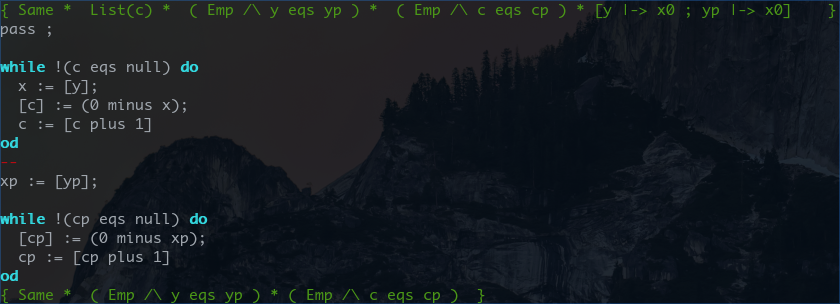
\includegraphics[width=\linewidth]{pictures/CLI.png}
		\caption{Formatted output of the prover}
		\label{fig:CLIScreenShot}
	\end{figure}
	\item The \texttt{metaPrettyPrint} operator in the \texttt{META-LEVEL} module, which returns a term as a list of quoted identifiers to be printed, formatted respecting the \texttt{format} attributes defined for the operators used in the term. An example is presented in Listing \ref{takeFirst}, which presents the rule used to take the top element of the \textbf{GoalStack} for processing, and writes the formatted output of the goal to the \textbf{StagingOutput} field.
	\begin{figure}[h]
	\begin{lstlisting}[label=takeFirst,caption=Rewrite rule making use of metaPrettyPrint]
crl [takeFirstGoalFromList] : < noAction ; RG ; noGoal ; G <> GS ; GL ; nil > 
=> 
< check ; RG ; G ; GS ; GL ; 'current ' 'goal '  '  'is '\n metaPrettyPrint(upModule('PROVER-INTERFACE, false), upTerm(G)) '\n > 
if G =/= noGoal .
	\end{lstlisting}
	\end{figure}
\end{itemize}
All throughout the prover calls to \texttt{metaPrettyPrint} have been made in order to inform the user of what the prover is doing and how.
\\

For a more advanced user interface or to expose the prover's functionalities through a programming interface, a wrapper written in more feature-rich language through which to control the Maude environment is probably the best choice. The concept is exemplified by the Maude plug-in for Eclipse, \cite{maudeEclipsePLugin} which enables writing of Maude code inside the Eclipse IDE, and the plug-in communicates with the underlying Maude environment. The project also includes a plug-in which allows any Java program to communicate with Maude.
\section*{Conclusions}
The development of the Relational Separation Logic prover helped us get a deeper understating of it, along with an introduction to other theoretical concepts used in program analysis and programming language semantics, such as Separation Logic and Rewriting Logic.
\\

While the two Separation Logics used throughout the paper are powerful tools for analyzing the behavior of program and are relatively easy to understand, it takes time to become familiar with them and use the m at their full potential.
\\

The logics are better suited for studying small snippets of code and not entire programs, because the demonstration can get cumbersome and end up spending a lot of time on focusing on irrelevant parts of the program. 
\\

Maude has been interesting to work because it required an entirely different mindset than the other programming languages I was familiar with . Once getting grasping the concepts around Maude which was built, it was easy to come up with simple, clever solutions to the problems I was facing. As it is described on it's website \cite{maudesite}, Maude is a powerful logical framework which allows modeling of other logics in it; it proved to be exactly that, enabling us to represent the logics in a natural manner, which made the implementation much less error-prone and allowed us to focus on the relevant part of this project, namely how to apply the logics instead of focusing on how to properly implement them.
\\

While being a powerful and interesting language to work with, being a fairly specialized and not very widespread, guidance and help are limited to the manual \cite{maudeprimer} and \cite{manual}. This obstacle resulted in significant time spent on searching for solutions to otherwise trivial problems, especially when starting using the language, because the source of the problem is usually unclear to a beginner. 
\\

Overall, this whole project has been an interesting introduction to both  theoretical concepts regarding program analysis and new, different technologies. The mix of the two resulted in the built prover, which could be improved in the future with the features discussed throughout the chapters and others to easily accommodate real-world usage. 

\pagebreak
\bibliographystyle{unsrt}
\bibliography{bibliography}


\end{document}